\subsubsection{Modelo GPIO}

El modelado de las entradas y salidas en una placa hardware (o emulada) con soporte \gls{gpio} es una de las partes más importante del dispositivo \gls{iot}. Mediante este componente, podremos interactuar con otros dispositivos externos tales como sensores digitales, analógicos, actuadores, etc.

La representación de los modelos, se hará en tres grupos lógicos para su mejor modelado y separación de tareas:  gpio, gpio events y gpio actuators.



En estos modelos definiremos de una forma abstracta estos conceptos para poder interactuar más adelante con ellos.

Los dispositivos \gls{gpio} cuentan con una serie de entradas analógicas o digitales. Muchos de ellos tienen entradas con múltiple funcionalidad pudiendo comportarse como entradas digitales o analógicas vía configuración en tiempo de ejecución. Así mismo, son capaces de funcionar en otras modalidades tales como \gls{rs232} o \gls{i2c}, compartiendo la misma entrega física entre las diversas opciones. Esto quiere decir, que podemos corromper hardware si por error cambiamos un valor de una variable en ejecución, algo que en un lenguaje general debería ser permitido, en nuestro \gls{dsl} no deberíamos dejar, con lo que nuestro programa sería válido en compilación.

Esta funcionalidad tan específica, deberá quedar fuera del modelo, debiéndose soportar en el código no generado automáticamente a partir de los modelos.

Debido a que posteriormente en la sección \gls{dsl} crearemos un lenguaje de tipado fuerte, modelaremos las entradas / salidas especificando el tipo de estas (digital / analógico), evitando posibles fallos en hardware si por ejemplo activamos una salida en un dispositivo de entrada (pudiendo incluso quemar el dispositivo sino incluye algún tipo de resistencia previa).

Otra funcionalidad igualmente importante es la capacidad que tienen estos dispositivos de generar interrupciones vía hardware en el momento de cambio de estado de la señal digital, algo necesario para nuestra definición posterior de sistema de eventos, soportado en mayor medida por este tipo de dispositivos.

En el caso de los sistemas que no posean la característica de interrupción vía hardware, deberá ser emulada mediante software realizando polling sobre el estado de la entrada en cuestión. En el caso de dispositivos con sistema operativo de propósito general como Raspberry PI, se realizará en el hilo principal. En el caso de Arduino, la consulta se realiza dentro del \gls{mainloop}.

Esta casuística de emulación de interrupción vía software no quedará definido en este meta-modelo sino que será definido en la implementación a código final de la plataforma en cuestión.

Nuestro modelo \gls{gpio}, cuenta con una serie de funcionalidades declarativas, permitiendo al desarrollador especificar una serie de tareas sin saber como en capas inferiores las realiza la plataforma. Podemos ver ejemplos como: ButtonInputAccumulator, evento por el cual cada vez que pulsamos un botón (cambiamos de estado durante un tiempo mínimo una entrada \gls{gpio}), lanzamos un evento con un contador de veces.

En la figura \ref{fig:modelo_iot_gpio_classes} podemos observar el diagrama de clases del modelo \gls{gpio} base, en la figura \ref{fig:modelo_iot_gpio_events_classes} mostramos los eventos generados por el dispositivo \gls{iot}. Por último, la figura \ref{fig:modelo_iot_gpio_actuators_classes} muestra los actuadores con los que contamos en el modelo. 

\begin{figure}
	\centering
    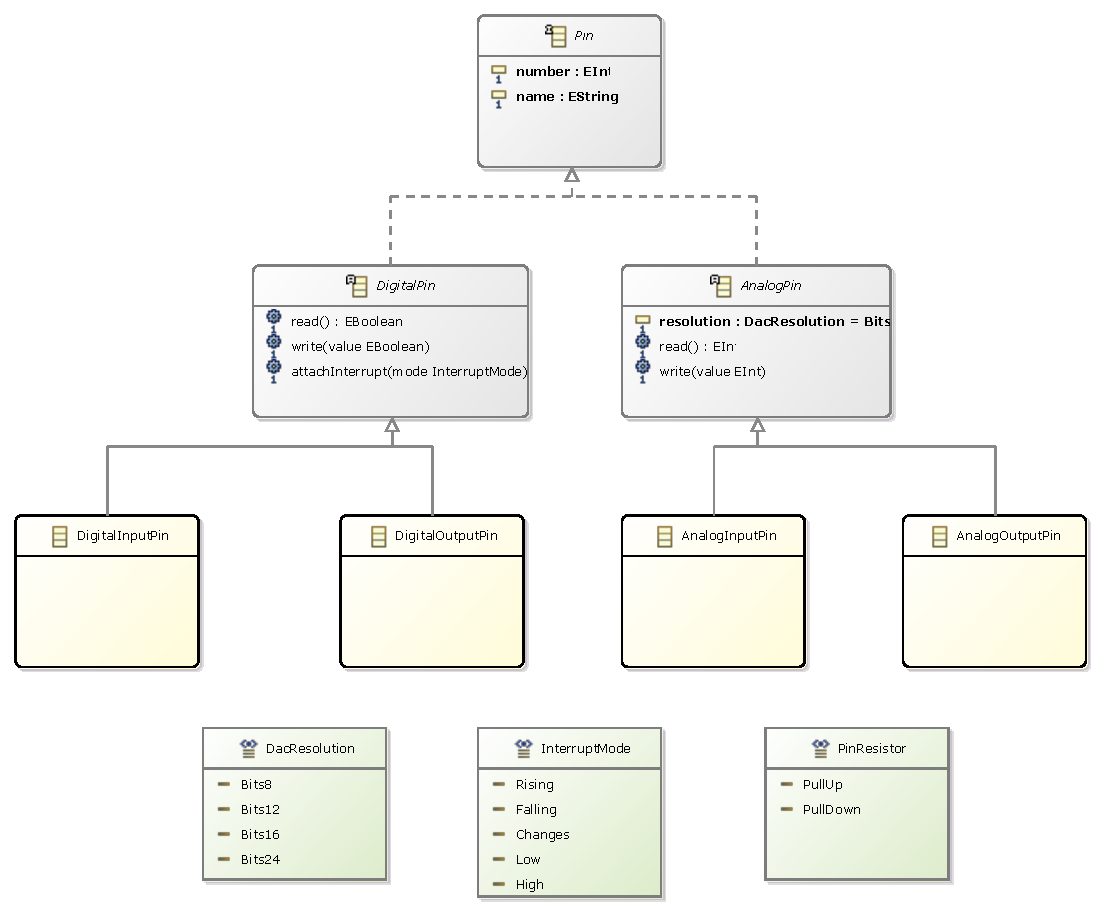
\includegraphics[height=0.3\textheight]{images/models/gpios_class_diagram.pdf}
    \captionmodeloclase{GPIO}
    \label{fig:modelo_iot_gpio_classes}
\end{figure}

\begin{figure}
	\centering
    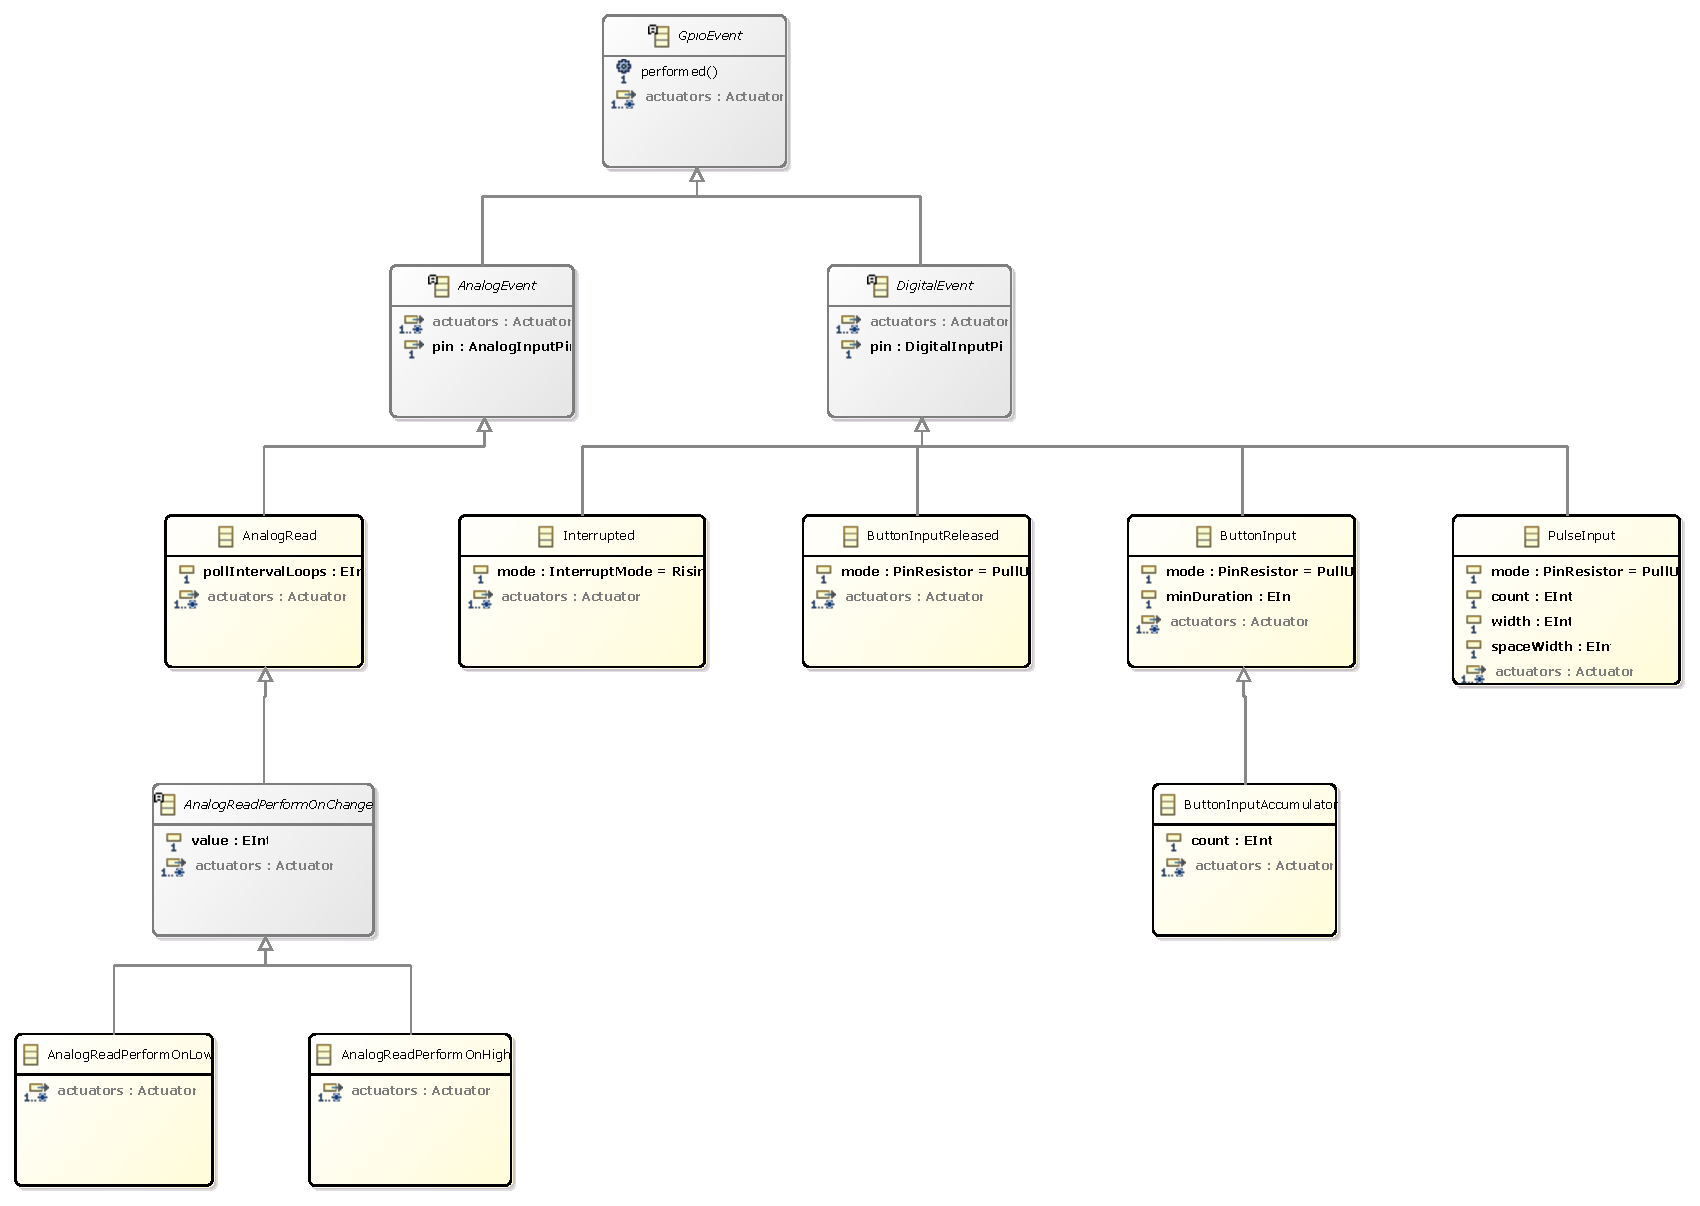
\includegraphics[height=0.3\textheight]{images/models/gpiosevents_class_diagram.pdf}
    \captionmodeloclase{GPIO - Eventos}
    \label{fig:modelo_iot_gpio_events_classes}
\end{figure}

\begin{figure}
	\centering
    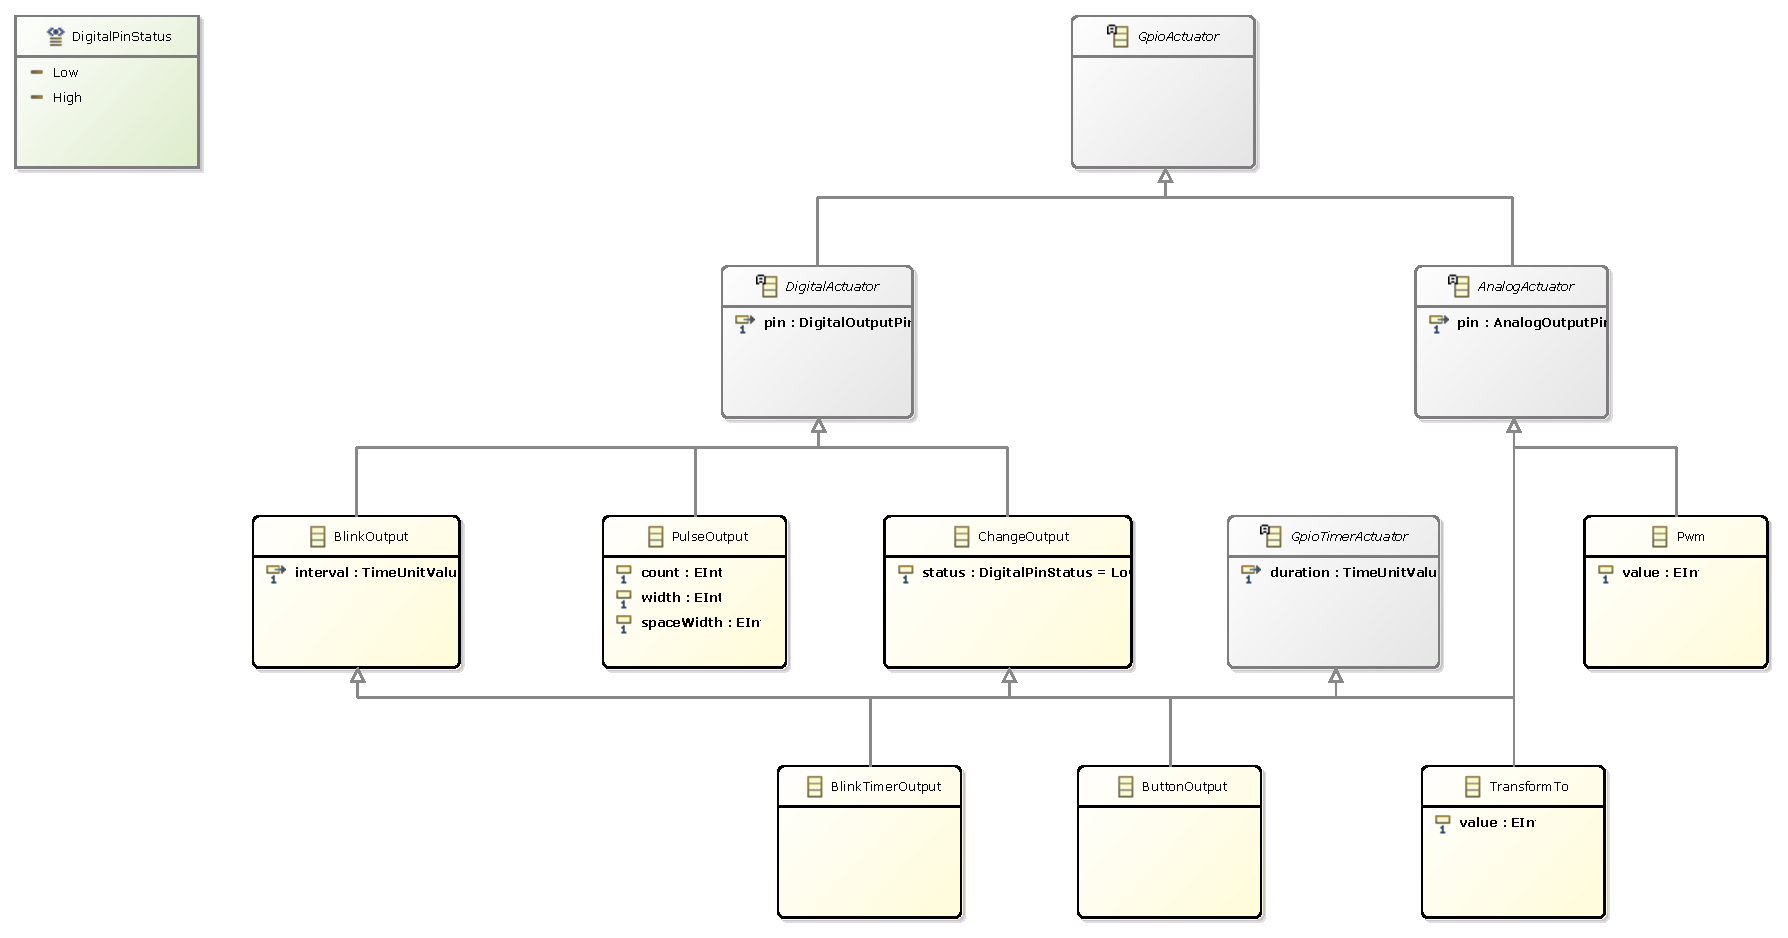
\includegraphics[height=0.3\textheight]{images/models/gpiosactuators_class_diagram.pdf}
    \captionmodeloclase{GPIO - Actuadores}
    \label{fig:modelo_iot_gpio_actuators_classes}
\end{figure}
